{\large{Compra de materiales}} \\
{\bf{Descripción:}} \\
Flujo operativo cuando se realiza una solicitud de compra de materiales. Este proceso va desde el origen de la necesidad de compra, hasta que se realiza el pago de la misma. \\

{\large{Control de entradas de inventario}} \\
{\bf{Descripción:}} \\
Definir exactamente los pasos que deben hacerse para ingresar un producto en elstock de la empresa. \\

{\large{Pedido de venta de producto, transporte propio}} \\
{\bf{Descripción:}} \\
Flujo operativo cuando un cliente realiza un pedido de ventas, y en su expedición se utiliza un transportista contratado por nosotros mismos. \\

{\large{Proceso de cobro de facturas}} \\
{\bf{Descripción:}} \\
Flujo operativo de un cobro de factura. En el proceso actual hay una serie de particularidades, como cheques posdatados (que pueden endosarse para pagar proveedores), y otros documentos de compra que pueden utilizarse para aplicar cobros de clientes.


\begin{center}
 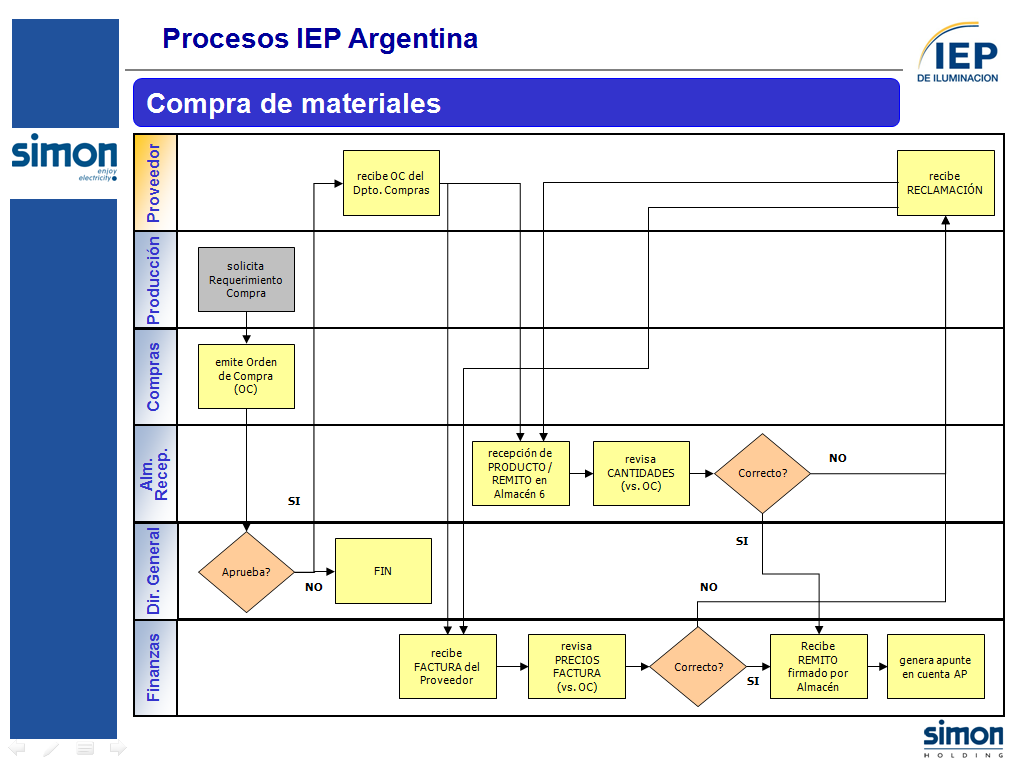
\includegraphics[angle=90,scale=0.80,keepaspectratio=true]{./Images/Procesos-Circuitos-Originales-IEP/Circuito-Compras-IEP.PNG}
 % Circuito-Compras-IEP.PNG: 1024x768 pixel, 96dpi, 27.10x20.32 cm, bb=0 0 768 576
\end{center}

\begin{center}
 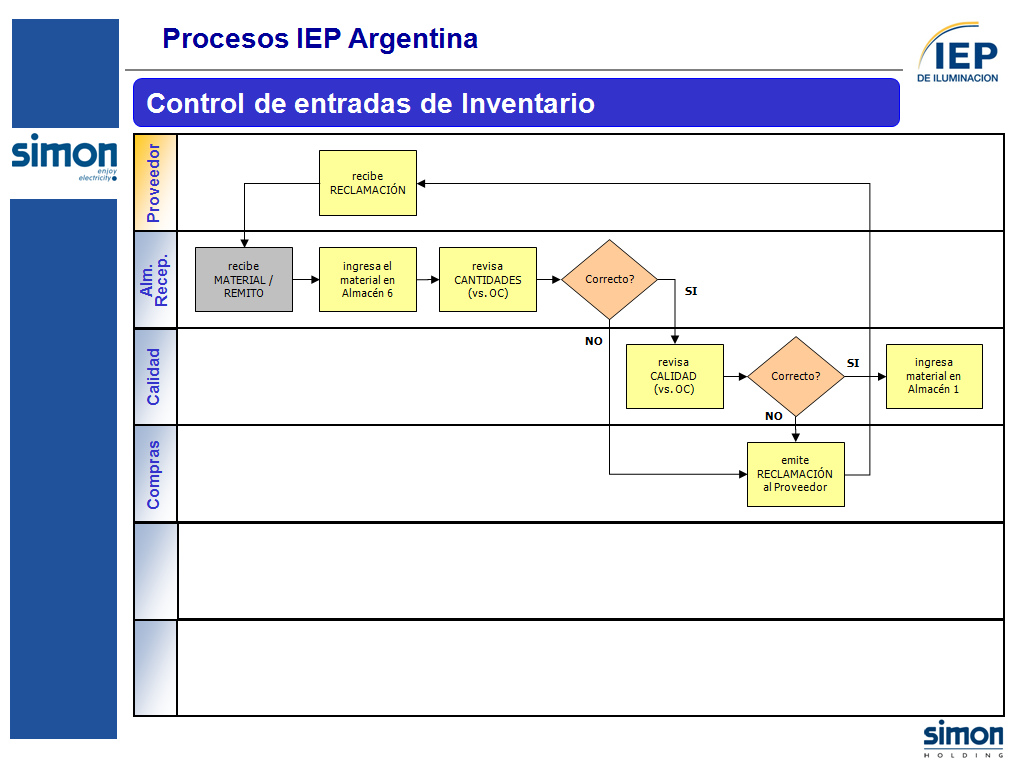
\includegraphics[angle=90,scale=0.80,keepaspectratio=true]{./Images/Procesos-Circuitos-Originales-IEP/Circuito-Compras2-IEP.PNG}
 % Circuito-Compras2-IEP.PNG: 1024x768 pixel, 96dpi, 27.10x20.32 cm, bb=0 0 768 576
\end{center}

\begin{center}
 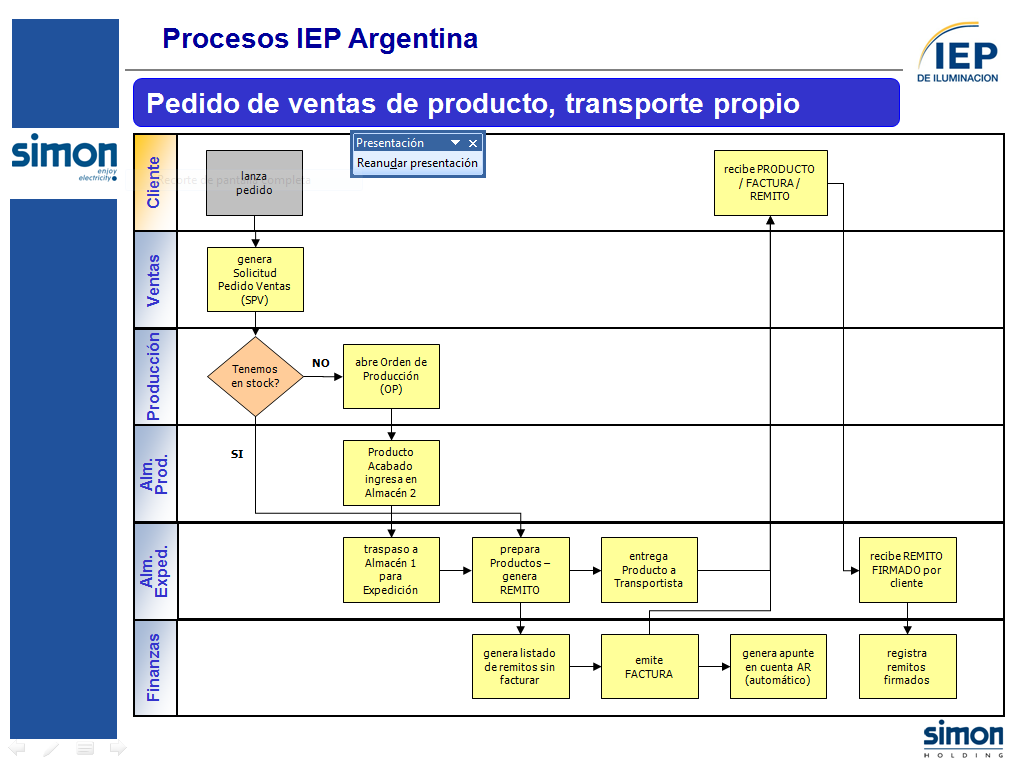
\includegraphics[angle=90,scale=0.80,keepaspectratio=true]{./Images/Procesos-Circuitos-Originales-IEP/Circuito-Ventas-IEP.PNG}
 % Circuito-Ventas-IEP.PNG: 1024x768 pixel, 96dpi, 27.10x20.32 cm, bb=0 0 768 576
\end{center}

\begin{center}
 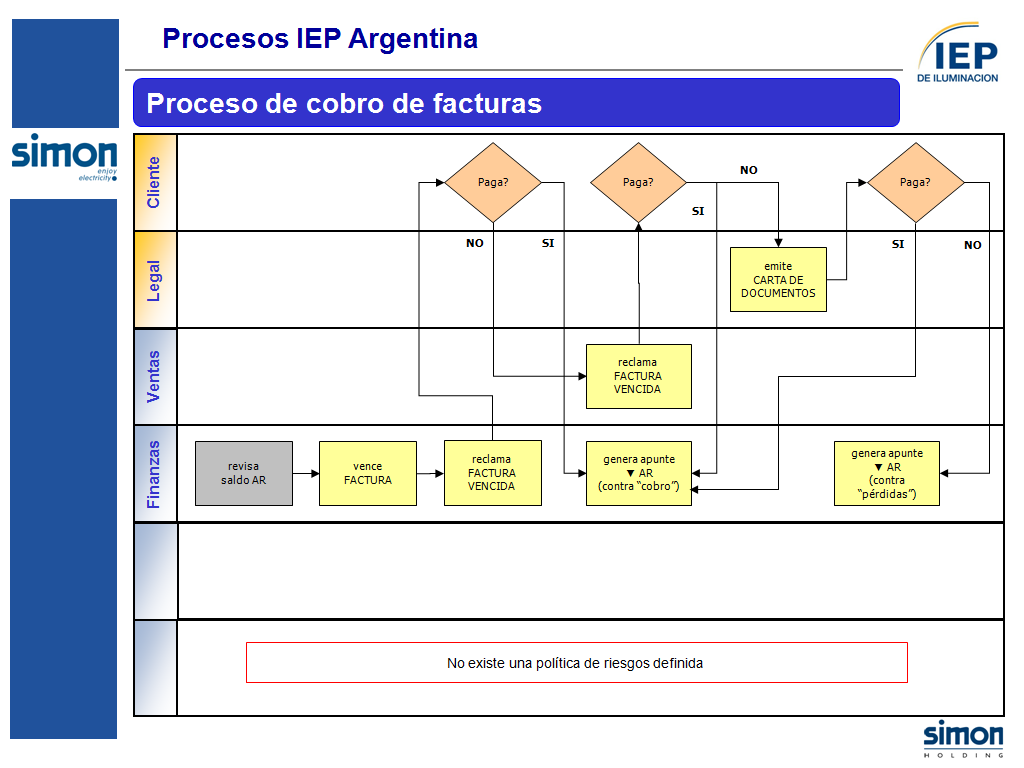
\includegraphics[angle=90,scale=0.80,keepaspectratio=true]{./Images/Procesos-Circuitos-Originales-IEP/Circuito-Cobranzas-IEP.PNG}
 % Circuito-Cobranzas-IEP.PNG: 1024x768 pixel, 96dpi, 27.10x20.32 cm, bb=0 0 768 576
\end{center}
